\documentclass{IEEEtran}
\usepackage[utf8]{inputenc}
\usepackage{graphicx}
\usepackage[toc,page]{appendix}
\graphicspath{ {./images/} }

\title{Ransomware: Malicious Encryption}
\author{Colton Alseth}
\date{October 2018}

\begin{document}
\pagestyle{plain}
\bibliographystyle{plain}

\maketitle
\begin{abstract}
    ~Ransomware has proven to be a powerful form of malware. The main concept behind ransomware is to restrict a victims access to their computer, and then use that to extort them for money. The first iteration of ransomware in 1989 was unsuccessful. Yet, the idea was novel and provided a proof-of-concept. The concept was later adapted to include better techniques and technologies. Different encryption techniques were employed to make it more effective. Eventually, ransomware became one of the most effective forms of malware. It reached a peak number of attacks in 2016, but the total number of attacks dropped between 2016 and 2017. However, this trend is not guaranteed to continue. Ransomware will likely continue adapt to adversity. To give a complete understanding of ransomware, this paper explores its history, its inner-workings, and its possible future adaptations.
\end{abstract}

\tableofcontents

\listoffigures

\section{Introduction}

A common way to exploit computers is through the employment of malicious software, which is commonly referred to as \textbf{malware}. There are various types of malware, including viruses, worms, trojan horses and spyware. However, there is another type of malware which has become more prevalent in recent years. It is known as \textbf{ransomware}, and its concept is simple: attack users by restricting their access to their computer, and use this to extort them for money in exchange for restoring their system. It is a way for an attacker to target an individual or group, and receive payment with relatively little effort. The most popular way this is done by encrypting a user's files. Assuming the victim has files they care about, they will feel compelled to pay the ransom to recover them. Ransomware's initial iteration was ineffective due to limitations in technology at the time. However, ransomware continued to evolve and utilize emerging technologies where necessary, until it became an effective style of malware. Now, it has become a popular variety due to its unique ability to directly extort money from victims. Ransomware has adapted to its weaknesses over the years and has gradually become more robust and sophisticated. This paper is an overview of ransomware, covering its history and adoption of certain technologies, how it uses encryption to be effective, and where we think it may prove to be troublesome in the future.


\section{Historical Survey}

Ransomware is perceived as a modern problem due to its recent widespread success, but it was first used almost three decades ago. The first iteration of ransomware appeared in 1989. It was known as the "AIDS Trojan," and was created by Dr. Joseph Popp, an evolutionary biologist~\cite{RN40}. This initial piece of ransomware provided a proof-of-concept, yet fell short of being effective in different ways. Personal computers and the Internet were still both relatively obscure tools at them time, so the technologies necessary to execute a successful anonymous attack weren't available yet. Today, certain technologies and software have been developed that allow ransomware attacks to be very effective.

\subsection{Encryption}\label{encryption}
When examining the potential effectiveness a piece of ransomware, the process of encrypting victims files is the most important aspect to consider. If file encryption is not effective, then the rest of the process would be for nothing. To encrypt the files on a victim's computer with the AIDS Trojan, Popp used a symmetric encryption algorithm (symmetric encryption will be discussed more in Section~\ref{symenc}). Due to the nature of symmetric encryption, the encryption key needed to be embedded in the ransomware source code when it was created. This made it possible for victims to examine the software and extract the key to decrypt their files without ever paying the ransom. It may have frightened those affected, but it was not effective at getting them to pay the ransom. Many were able to successfully restore their systems without having paid the ransom~\cite{RN40}. The choice of encryption was a significant shortcoming of the AIDS Trojan.

Researchers at Columbia University took the idea of the AIDS Trojan and expanded on it in 1995. They wanted to further explore how cryptography could be used maliciously. They came up with a concept, which they referred to as “cryptoviral extortion,” that is the basis for most modern ransomware. They understood the issues that the AIDS Trojan faced, so their concept also incorporated asymmetric encryption (asymmetric encryption will be discussed more in Section~\ref{asymenc})~\cite{RN24}. Incorporating asymmetric encryption was a significant moment in the history of ransomware. It is \textit{the} vital technology in making ransomware attack victims helpless, by removing any chance at accessing the decryption key. The concept was met with some skepticism, claiming it would never be a significant issue. However, the idea of using asymmetric encryption for electronic extortion would prove its effectiveness within the next few decades.

Ransomware's first public iterations using this scheme came in 2006 with Gpcode, Cryzip, and Krotten. They used RSA encryption as their asymmetric encryption algorithms, and employed various key sizes: 56-bit, 330-bit, and 660-bit. These forms of ransomware did not employ strong enough encryption to be effective. Encryption with those sized keys was reversed in a reasonable amount of time, with a reasonable amount of computing power~\cite{RN22}. However, more strains continued to appear, and by 2008 a variation of Gpcode called Gpcode.AK was discovered to be using a 1024-bit key. This made it nearly impossible to compute the key in a reasonable amount of time. For example, it was estimated it would take approximately 15 million computers (with average compute power at the time) one year to discover~\cite{RN21}. Simply by increasing the encryption key size, the developers escalated ransomware's risk level from nuisance to threatening.


\subsection{Communication}\label{communication}
The method of distribution for the AIDS Trojan was done physically by putting the software on floppy disks. Dr. Joseph Popp distributed the disks to twenty-thousand World Health Organization~(WHO) doctors via mail under the guise it was AIDS education software. To unlock their systems after they had been encrypted, the WHO doctors needed a specific piece of decryption software written by Dr. Popp. And in order to obtain it, they were instructed to send the payment to a Panamanian PO Box~\cite{RN40}. This was another mistake made Dr. Popp. This process was not an anonymous way to conduct communication between the attacker and victim. By giving out personal information, such as a PO box, he was providing details that could later be linked to him. With the advent of the Internet, communication and the distribution on software between the attacker and the victim became more efficient. However, it didn't solve the anonymization issue. Some information, like IP addresses, could be traced back to the attacker and they could be tracked down or taken offline. Without anonymity, using extortion software would be too risky for an attacker~\cite{RN33}.

To address the issue of anonymous communication, certain types of ransomware have been identified using the Tor network for communication. Tor masks a user's identity because it uses a network of thousands of servers, or relays, around the world to obfuscate the link between the client and server. When a client makes a request, a series of randomly selected relays pass that information between each other and ultimately to the server. The response from the server is then sent back through the same path of relays, eventually returning the information to the client. The data packets between relays are also encrypted, so each relay only knows which relay it came from and which one it goes to next. Additionally, when information reaches its destination over the Tor network, the computer receiving the information has no way of knowing where that request came from because the IP address of the sender is not included in the packet~\cite{RN39}. Tor is a safe and effective way for attackers to communicate with victims. Attackers would be able to exchange necessary information without having to worry about that communication being traced back to them.
 
Additionally, many modern forms of ransomware use command-and-control~(C\&C) servers operating on the Tor network. These servers are who the victim is actually communicating with when they are attempting to get the decryption key to recover their system. Everything is automated on the command-and-control server, which improves efficiency for the attacker and makes large-scale attacks possible. When a specific victim pays their ransom, the server is able to keep track of which key to send back to them based on the details of their computer, such as their IP address, or a unique identifier generated by the ransomware~\cite{RN33}.

Tor has proven to be a valuable technology in the execution of ransomware attacks. Tor was first released in 2002. However, the first piece of ransomware, known as Onion, using Tor for anonymous communication was identified in 2014~\cite{RN39}\cite{RN37}. Since that time, around three-quarters of all ransomware has been identified using some form of anonymization and services for secure communication~\cite{RN33}.

\subsection{Payment}\label{payment}
After their systems were compromised, the doctors from the World Health Organization were given a prompt by the malware stating they would need to pay to recover their system. They were told to make payments out to a shell company owned by Dr. Popp~\cite{RN40}. Again, this provided personal information about the attacker. By giving the victims a company name to pay to, Dr. Popp was leading the investigation back to himself. However, at the time, and for the following two decades, this was the only practical way for someone to receive a ransom. The money would have to somehow be transferred physically between the attacker and the victim, or it would have to go through conventional monetary systems, using a wire transfer or prepaid debit cards. There were no viable options for receiving a ransom that would not expose some of the attacker's information.

In January of 2009, an unknown person, or group, by the name of Satoshi Nakamoto released the Bitcoin protocol publicly. Bitcoin is peer-to-peer network, that facilitates the exchange of the electronic currency known as \textbf{bitcoins}. The protocol uses asymmetric encryption to work. The public key acts as an outward facing address for Bitcoins to be sent to, while the private key is used to sign off on transactions. One of the hallmark features of Bitcoin is that its transactions can happen pseudonymously. Bitcoin key pairs are assigned randomly and have no significance other than allowing transactions to take place~\cite{RN36}. This means that the public address can't easily be traced back to a specific person. The transactions going to and from an address can be monitored, but it is difficult to extract other information directly from those transactions. The combination of relative anonymity and simplicity from Bitcoin transactions would eventually provide a powerful way of paying ransoms.

Bitcoin was not necessarily intended to be used in this way, but all of its characteristics lend it to be used for transactions like this. Bitcoin was meant to be a "trustless" form of payment, where neither side had to know or trust their counterparty. Bitcoin simply guaranteed the person receiving payment would certainly get their money if a transaction to them was created. When a payment happens, the payer must have enough Bitcoin in their wallet and once the money is sent, there is no way to recover that money as no third-party mediates the transaction~\cite{RN36}.

Bitcoin was only used by a small number of people for the first few years and didn't carry significant monetary value during that time. Asking for a ransom in Bitcoin didn't make sense initially, and would have been difficult for the victim to figure out. However, after a few years, the system proved effective and bitcoins continued to gain in dollar value. Around 2013 the use of Bitcoin for ransom payments became common. The first piece of ransomware to do so was known as CryptoLocker. It successfully extorted around \$27 million in bitcoins from victims~\cite{RN34}. Just like the use of the Tor network, it became ubiquitous and around three-quarters of all ransomware attacks since have requested cryptocurrency for payment~\cite{RN33}.


\section{Technical Underpinnings}\label{techund}

\subsection{The Five Stages of An Attack}\label{overview}
Ransomware attacks are typically broken into five different stages. All steps are important to successfully complete a ransomware attack. The stages are:
\hfill \break

\begin{enumerate}

    \item \textbf{Exploitation and infection:} Ransomware must be delivered to the victim's computer in some way. Typically, this is done with a phishing e-mail or by using an exploit kit. An exploit kit finds vulnerabilities in software, like Adobe Flash or Internet Explorer, through outdated or insecure software, with the intention of spreading malware.
    \item \textbf{Execution:} Once a computer has been compromised, the malicious software is executed on the system. When ransomware begins executing, it typically starts by creating persistence mechanisms. So, if the computer is shut off in the middle of execution, it continues the process where it left off once the computer starts again.
    \item \textbf{Backup spoliation:} At this stage, it attempts to search the system for backups. If any are found, the ransomware deletes them from the system to prevent recovery without paying the ransom. Since ransomware is entirely dependent on the victim being unable to access their files, this is a vital step.
    \item \textbf{File encryption:}\label{step4} Once persistence mechanisms are in place and back-ups are deleted, it can begin encrypting the files on the system. First, it gives the system a unique identifier and then exchanges encryption keys with a Command-and-Control (C\&C) server. The ransomware then begins encrypting the computer's files. Depending on the type of encryption, this process can vary in duration. Typically, this process is short.
    \item \textbf{User notification and clean-up:} Finally, the ransom note is posted on the victims' computer. This usually includes some information about what has happened and instructions on how the user can recover their system. The ransomware then removes itself from the victims' computer. This is done so that the ransomware cannot be studied and understood for preventing future attacks.
\end{enumerate}


These five stages make up the entirety of a ransomware attack~\cite{RN29}. \textbf{Step~\ref{step4}} is the most important. If the encryption scheme fails, is too weak, or the keys are found by the victim, the entire attack falls apart. The main focus of Section~\ref{techund} will be on this step and the types of encryption that allow it to work.

\subsection{Encryption Types}\label{encryption}
Knowledge of certain terminology will be needed to understand the two types of encryption. Here is a list of terms to understand and refer back to as necessary while reading through this paper:
\begin{itemize}
    \item \textbf{\textit{Encryption:}} The process of taking human-readable information and turning it into gibberish. The encryption process requires an encryption key and an algorithm, which is the explicit process of using the key to encrypt the information.
    \item \textbf{\textit{Decryption:}} The process of taking the gibberish and turning it back into human-readable information. The decryption process requires a decryption key and an algorithm, which is the explicit process of using the key to decrypt the data.
    \item \textbf{\textit{Plaintext:}} The human-readable form of information. This is the information that can be encrypted so that it can no longer be easily understood. Encrypting plaintext gives you ciphertext.
    \item \textbf{\textit{Ciphertext:}} The encrypted form of information. This is typically not in a readable form and requires a key to be put back into a form that can be understood. Decrypting ciphertext gives you plaintext.
    \item \textbf{\textit{Encryption Key:}} The value(s) applied in the encryption algorithm to create ciphertext from plaintext.
    \item \textbf{\textit{Decryption Key:}} The value(s) applied in the decryption algorithm to get back to plaintext from ciphertext.
\end{itemize}

There are two primary categories that cryptographic algorithms fall into: symmetric and asymmetric~\cite{RN20}. \hfill \break

\subsubsection{Symmetric Encryption}\label{symenc}
Symmetric encryption has a single key that acts as its encryption key and its decryption key. A symmetric encryption key is used to encrypt plaintext and decrypt ciphertext. 

\begin{figure}[h]
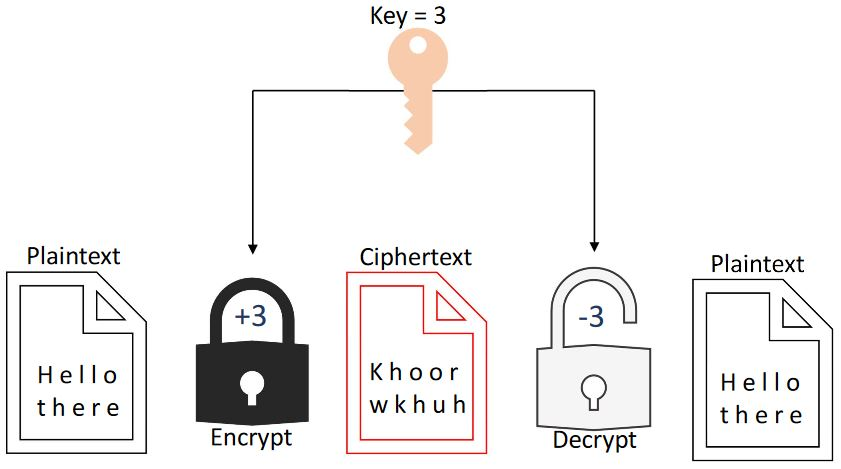
\includegraphics[width=\linewidth]{se.JPG}
  \caption{A simplified example of symmetric encryption that has a key of 3. Symmetric encryption uses the same key for encryption and decryption. For this example, encryption shifts each character in the plaintext forward in the alphabet by the key, and decryption shifts each character from the ciphertext backward in the alphabet by the key.}
  \label{fig:symenc}
\end{figure}

If an encryption algorithm \textit{E} is being used to encrypt a piece of plaintext \textit{T} with a given key of \textit{K}, it produces ciphertext \textit{C}:

\[C = E_K(T) \]\label{eq1} 
In symmetric encryption, the decryption process of going from ciphertext back to plaintext uses the inverse of the encryption algorithm. If the decryption algorithm \textit{\(E^-^1\)} is being used to decrypt the piece of ciphertext \textit{C} that was just created, using the same key \textit{K} as before, it produces the plaintext \textit{T} that was started with:

\[T = E_K^-^1(C) \]\label{eq2}
This is how symmetric encryption and decryption work in theory~\cite{RN30}. To get a better understanding of how this may work look practice, refer to Fig.~\ref{fig:symenc}. 


Symmetric encryption has certain strengths and weaknesses. One of the main benefits of symmetric encryption is its efficiency. Symmetric encryption and decryption algorithms work quickly. They are not typically computationally demanding to do. This property would greatly benefit anyone attempting to create a piece of ransomware. Because ransomware is usually encrypting many different files on the victim's computer, it needs to be done in the least time possible. This gives the victim less time to react and find a way to stop the execution.

However, one of the significant downsides of symmetric encryption is that it is less secure. This does not mean the encryption is easy to crack, instead it is related to its single key design. Since the same key is used for encryption and decryption, it is impossible to keep the decryption key hidden from the victim using symmetric encryption alone. As soon as the key is used in plaintext on the victim's computer, encryption can be easily broken. The key can be used to simply decrypt any piece of data that it encrypted~\cite{RN20}. For ransomware's purposes, this is a trait that is can't be ignored. Symmetric encryption is not effective for ransomware by itself.

One of the most common algorithms for symmetric encryption is the Advanced Encryption Standard (AES). The algorithm was proposed by Vincent Rijmen and Joan Daemen, two Belgian cryptographers, in 1998. AES was recommended to be the symmetric encryption standard by the US National Institute of Standards and Technology, replacing the Data Encryption Standard (DES). AES has a  variable key length, that must be a multiple of 32, a minimum of 128 and a maximum of 256. The larger the key, the more difficult it is to reverse the encryption process without knowing what the key is, and the less ~\cite{RN20}. AES has continued to be the standard for symmetric encryption and has been used by many variants of ransomware in the past~\cite{RN25,RN33}. 

\subsubsection{Asymmetric Encryption}\label{asymenc}

In asymmetric encryption, or public-key encryption, there are two separate keys. There is a private key, which should only be known by the person who generated it. The private key is also typically used for decrypting ciphertext. The public key, which is derived from the private key, can be used by anyone to encrypt a piece of plaintext. This separation allows the generator of the keys to distribute the public key to anyone without worrying about the encryption being broken. It is difficult to break public key encryption without knowing the private key. Having two distinct keys allows the creator to hold the private key, while freely giving out the public key. This ensures that they are the only one who is able to decrypt any information encrypted using their public key~\cite{RN20}. Fig.~\ref{fig:asymenc} shows how asymmetric encryption works conceptually.


\begin{figure}[h]
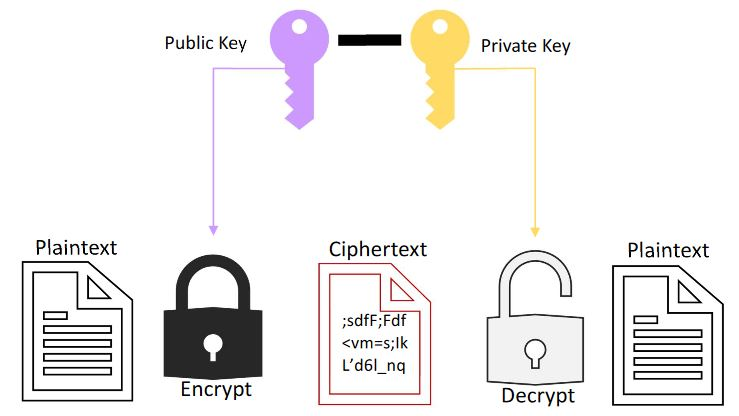
\includegraphics[width=\linewidth]{ae.JPG}
  \caption{A general look at how asymmetric encryption works. Plaintext is encrypted using the public key and the ciphertext is decrypted using the private key. The public key is derived from the private key. }
  \label{fig:asymenc}
\end{figure}

It's beneficial to see how a key pair may be generated and how that key pair can be used for encryption and decryption. As an example, the Rivest–Shamir–Adleman (RSA) encryption algorithm will be used to show how the process works. RSA encryption is named after Ron Rivest, Adi Shamir, and Leonard Adleman, who first described the algorithm in 1978~\cite{RN28}. RSA encryption is a common asymmetric encryption algorithm, and has been used by various types of ransomware in the past~\cite{RN25,RN21,RN22,RN26,RN14}.

There are two algorithms that are given in RSA encryption. The first is the encryption algorithm, where \textit{C} is the ciphertext and \textit{T} is the plaintext:

\[C = T^e(mod~n) \]\label{eq3}
Next, the decryption algorithm:

\[T = C^d(mod~n) \]\label{eq4}
The plaintext is known in the encryption algorithm, and the ciphertext is known in the decryption algorithm. \textit{e} along with \textit{n} are the encryption key, and \textit{d} along with \textit{n} are decryption key. These values must be found to encrypt any plaintext, or decrypt any ciphertext.

A private key is created by simply choosing two prime numbers. For our purposes, one number is assigned to \textit{p} and the other to \textit{q}. Next, we find \textit{n}. \textit{n} is computed by multiplying \textit{p} and \textit{q} together:

\[n = p * q \]\label{eq5}

Assuming \textit{p} and \textit{q} are large enough, this makes the factorization of semi-prime \textit{n} extremely difficult. It should take long enough that it would be impractical to attempt. This is important, with \textit{n} being a part of the public key, which can be seen by anyone.

Next, the value for \textit{e} is found. To find \textit{e}, the following requirement \textit{R} is calculated first:

\[R = (p-1)(q-1) \]\label{eq6}

Once \textit{R} is known, a value for \textit{e} can be simply chosen, but it is required that it be relatively prime with \textit{R}. This means that they must not share a common factor other than one. This ensures that each value of plaintext has a unique ciphertext.

With all of the values for encryption generated, the values necessary for decryption should be computed next. Even though \textit{p} and \textit{q} are the private keys, they aren't used directly in the decryption algorithm. That value is \textit{d}, which is found by using \textit{p} and \textit{q} as well as \textit{e}:

\[e * d =  1~(mod~(p-1)(q-1))\]
Without \textit{p} and \textit{q}, \textit{d} is difficult to find. However, once it is found, decryption can now easily be done~\cite{RN28}. For an example of this entire process, refer to Fig.~\ref{fig:asymenc1}.

Asymmetric encryption's main strength is its two key design. Separating the encryption key from the decryption key allows them to be used independently of one another. This property is valuable for creating ransomware. The encryption key can now be embedded in the ransomware. Even if the victim is able to recover this key, they won't be able to decrypt their files with it. They are still dependent on the attacker who holds the private key to decrypt their files.

Asymmetric encryption is not wittout its own drawbacks, however. The main downside to asymmetric encryption is its tendency to be computationally expensive. A piece of ransomware may have to encrypt a large number of files, so it is important that this process is as short as possible. Again, this will give the victim less time to stop execution. Asymmetric encryption alone would simply be too slow to encrypt a large number of files on a victims computer.

\begin{figure}[h]
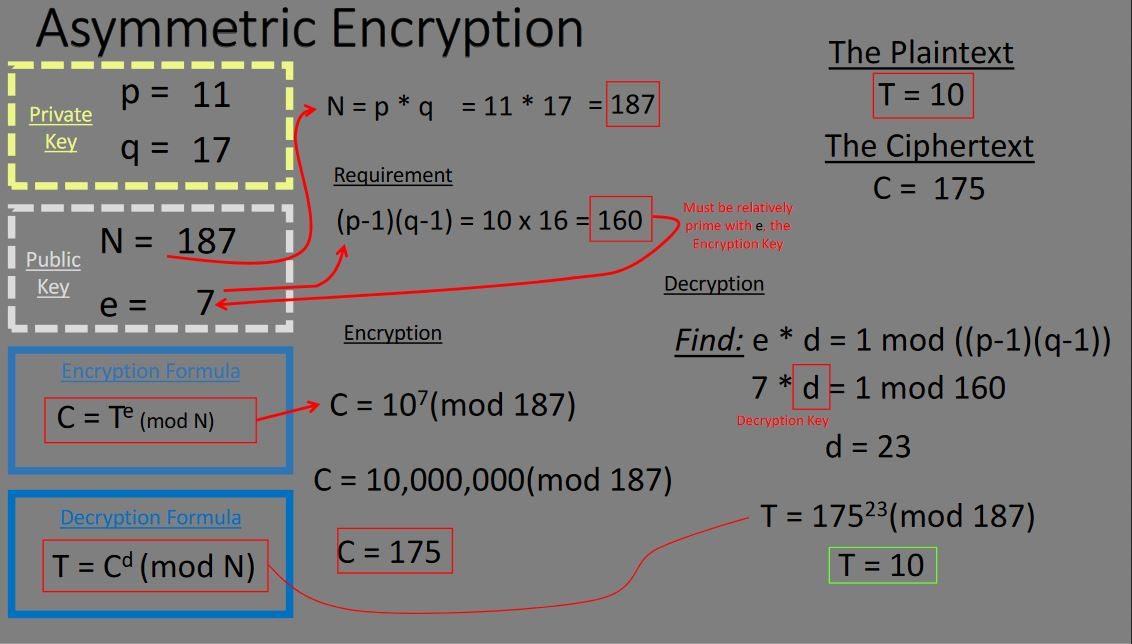
\includegraphics[width=\linewidth]{ae-ex.JPG}
  \caption{An example of asymmetric encryption that is encrypting a piece of plaintext with the value 10. First, it begins by choosing two prime values, 11 and 17, for the private key. Next, the values for the public key are found. (\textbf{Note}: All values in this example are much smaller than they would really be.)}
  \label{fig:asymenc1}
\end{figure}

\subsubsection{Cryptoviral Extortion}\label{crypext}

The power of encryption becomes more apparent when symmetric and asymmetric encryption are combined to leverage both their strengths and mitigate their weaknesses. In the context of ransomware, a symmetric key would be used to encrypt the victim's system files efficiently, while an asymmetric key pair would be used to make the victim reliant on the attacker. This is the process of \textbf{Cryptoviral Extortion}, which has three steps: 
\begin{enumerate}
    \item The attacker would pre-generate a pair of keys with an asymmetric algorithm, keeping the private decryption key and embedding the public encryption key in the code of the ransomware.

    \item Next, the attacker would find a victim and get them to execute the ransomware on their computer. This is generally done through phishing~\cite{RN28}. Once the ransomware begins executing, it generates a random symmetric key. It would then encrypt all files using the randomly generated symmetric key. Then the symmetric key would be encrypted using the public key from the pre-generated key pair.
 
    \item  Finally, the ransomware would purge the plaintext symmetric key from memory. The victim is left with ciphertext of the symmetric key and a way to contact the attacker. The only way to recover their files is to send that ciphertext to the attacker along with the requested ransom. The attacker would decrypt the ciphertext using the private decryption key, and send the plaintext symmetric key back to the victim allowing them to decrypt their files.
\end{enumerate}

This scheme, and slight variations of it, is what modern forms of ransomware use to be effective~\cite{RN24}. The speed of symmetric encryption and the secure, two key design of asymmetric encryption combine to create an encryption scheme that is difficult to break. The process makes the victim entirely dependent on the attacker. In Step 2, the encrypted symmetric key is no longer useful to them. It can't decrypt their files, and the public key can't decrypt the encrypted symmetric key. The process would never expose the private key to the victim, making them helpless without the attacker’s cooperation.

\section{Future Trends}

In 2016, known as "The Year of Ransomware", the number of attacks totaled 638 million~\cite{RN17}. The amount of money paid to cybercriminals was \$209 million in the first quarter alone~\cite{RN14}. Obviously, ransomware has been very effective in the past, and 2016 is the best example of this. Presently, ransomware attacks are contained primarily to desktop operating systems. This has historically been the best platform to extort people for money. However, ransomware will likely become less effective over time on this platform, even though there is no reason to believe its presence on desktop platforms will disappear entirely. It will not work as effectively as it has in the past due to increased awareness of the threat and the continued development of better anti-virus software for these platforms. 

This conclusion is derived from the fact that ransomware attacks are already beginning to decline. With 2016 having the highest number of attacks within one year at 638 million, 2017 had a fraction of that with 184 million attacks. Even though this number is still large, it's no longer a significant portion of the total malware attacks in the year. In general, malware incidents have continued to increase over the years. Ransomware's decrease is not because cybercrime has gone down. According to cybersecurity company SonicWall, the total number of malware incidents increased from 7.87 billion in 2016 to 9.32 billion in 2017~\cite{RN15}. That means the percentage of malware attacks relating to ransomware dropped from 8.107\% in 2016 to 1.974\% in 2017. 

The concept behind ransomware has proven to be effective in the past, so it will continue to be a threat going forward. Criminals will continue to adapt to the environment that they are presented. As time goes on, however, the creators of ransomware will not likely be able to limit their attacks to desktop platforms. If this platform begins to have diminishing returns, other large platforms that haven't been significantly affected by ransomware yet will probably be targeted, due to their lack of hardening.

To get a sense of what platforms this may spill over into, we will look at other currently popular platforms besides desktops, as well as any platforms that may be popular in the future. Today, another popular platform besides desktop is the mobile platform. And as we look into the near future, an emerging platform is the Internet-of-Things~(IoT). We believe that as ransomware becomes less effective in its current state, it will adapt and new strains will begin to target both mobile and IoT devices.

\subsection{Mobile Devices}\label{mobile}
The mobile platform would primarily include smartphones, tablets, and wearables. There are two simple reasons we believe mobile ransomware could become an issue within the next few years: there have been cases of mobile ransomware in the past, and the platform is expected to grow.
\hfill \break

\subsubsection{Previous Cases}
Even though ransomware has typically targeted desktop platforms in the past, there have been instances of mobile attacks as well. Mobile ransomware is not a new idea, which shows that it is a feasible option for ransomware attacks in the future. In the past, mobile ransomware has mostly affected Android phones. The first form of mobile ransomware was seen in 2012 and was known as Genric.17.1762. Historically, mobile ransomware has worked by locking users out of their phone rather than encrypting their files. It is usually delivered via an application that would ask for administrative privileges. If the user was not informed about malware, they may see no issue in granting this permission. Once this permission is granted, device authentication credentials are changed, and the user would be given a prompt that they need to pay to get their new credentials~\cite{RN13}. This is a relatively simple way to carry out an attack, but it has been effective. Fig.~\ref{fig:mr} shows what a mobile ransom note may look like. 

\begin{figure}[h]
\begin{center}
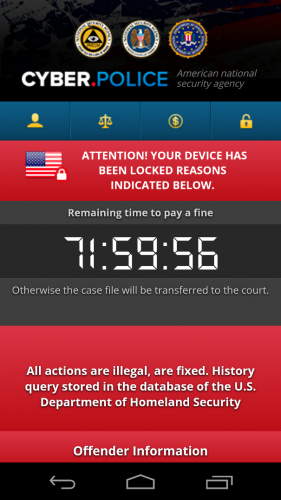
\includegraphics[scale = 0.4]{mobileransomware.png}
\end{center}
  \caption{A common ransom note on a mobile device. Typically, the note will say it is from a government agency and the user did something illegal. In order to make up for their crimes, the user must pay a fine. None of this is true, but it can scare victims into paying the ransom.
  (Picture from ~\cite{RN18})}
  \label{fig:mr}
\end{figure}

Development of mobile ransomware has not stopped, and new forms have continued to pop up. Due to the fact that mobile ransomware is already being used, it seems probable that its use will only expand in the future. In fact, despite ransomware's general decrease in use between 2016 and 2017, the number of mobile ransomware attacks increased by 250\% between the last quarter of 2016 and the first quarter of 2017~\cite{RN12}. This suggests that mobile ransomware may already be viewed as a viable alternative to desktop varieties, which is an idea that may push the creation of mobile ransomware going forward.
\hfill \break

\subsubsection{Platform Growth}
Mobile devices have become very popular in the modern world. It is uncommon to find someone who does not own either a smartphone, tablet or smartwatch. According to the Cisco Visual Networking Index~(VNI) as of 2015, in the United States alone, there were 447 million mobile devices in use. In addition, since they are not included in the main figure, there were also 34.9 million wearable devices in use. The number of mobile devices exceeded the population of the US, showing just how ubiquitous they have become. Cisco predicts that this number will increase dramatically over the next few years. They believe that there will be approximately 947 million mobile devices, as well as 163.2 million wearable devices by the year 2020~\cite{RN10}. That is more than double the total number of devices from 2015. 

Another interesting statistic compares the percentage of internet traffic from smartphones and PCs. Cisco states that currently desktop and laptop computers account for 41\% of total internet traffic, while smartphones only account for 18\%. However, they predict by the year 2022 these numbers will flip, with desktops accounting for 19\% of traffic, and smartphones accounting for 44\%~\cite{RN11}. These figures are important for illustrating how significant mobile platforms have become and will continue to be in the future. With the growth of the mobile platform, the use of desktop computers may decline.


\subsection{IoT Devices}\label{iot}
The Internet of Things is an emerging collection of smart-devices that connect to the internet. Generally, an IoT device is defined as an internet connected device that would not traditionally be connected to the internet. So devices like laptops, desktops, smartphones, and tablets would not be included. For consumer use, this would mostly include things you may find in a smart-home, such as smart fridges, smart thermostats, smart lighting, smart TVs and so on~\cite{RN9}. It extends beyond this for commercial uses in areas such as transportation for intercommunication between smart vehicles and traffic management, building automation to monitor and control the mechanical and electrical systems within a building, and healthcare for remote health monitoring and emergency notification~\cite{RN4}~\cite{RN3}. There are three primary reasons we believe IoT ransomware may become a reality in the next few years: the platform is expected to have significant growth, it currently has poor security, and proof-of-concepts demonstrate IoT ransomware's viability.
\hfill \break


\subsubsection{Platform Growth}
The range of uses for IoT is broad and will result in a large number of devices being manufactured. According to Gartner, the total number of IoT devices in use worldwide in 2017 was 8.38 billion. Consumer products made up the majority of devices in use with 5.24 billion. This is already a staggering number of IoT devices, but Gartner goes on to predict that by 2020 the total number of devices in use will be 20.41 billion, with 12.86 billion being consumer devices~\cite{RN8}. In the span of just three years, the total number of IoT devices will more than double. Like the mobile platform, but on an even greater scale, this will give cybercriminals a large attack surface for ransomware.
\hfill \break

\subsubsection{Poor Security}
Due to the interest in IoT devices growing at a rapid rate, manufacturers are looking to capitalize on this by rushing products to market. The downside to this is that security will often be neglected in favor of finalizing a product~\cite{RN2}. In fact, IoT security is already an issue. The best example of this is the Mirai botnet. In 2016, hackers were able to assemble a botnet of IoT devices by scanning the Internet for unsecured devices and then attempting to log in by using 61 common combinations of passwords and usernames. This was enough to create a botnet of about 500,000 devices. This botnet carried out a successful Distributed Denial of Service~(DDoS) attack against Dyn, which provides Domain Name System~(DNS) services to large companies such as GitHub, Twitter, Spotify, SoundCloud, Reddit, and the New York Times~\cite{RN5}~\cite{RN6}. Even though these attacks are not related to ransomware, they show that IoT devices can easily be exploited on a massive scale. If exploits are relatively simple on these devices, then it is only a matter of time before other malware attacks, including ransomware, begin to happen.
\hfill \break

\subsubsection{Proof-of-Concept}
Ransomware on IoT devices in not entirely speculative. There have been successful attempts to demonstrate that infecting IoT devices with ransomware is possible. A researcher from the security company Symantec was able to successfully infect their own smart TV with ransomware. The delivery was not done the traditional way with phishing, rather they used what is known as a Man-in-the-Middle~(MitM) attack. The researcher requested to download an application for their TV from an authorized server. This request was then intercepted by the researcher and redirected to a different server. The TV was no longer downloading an official application, but a malicious application that resembled the one requested. After running the infected application, certain permissions were granted to the application by the researcher, and the TV was successfully infected~\cite{RN7}. Even though this is just a proof-of-concept, it shows that infecting IoT devices with ransomware can happen and is something to be aware of in the future. 

\section{Conclusion}
Ransomware has evolved significantly from its first iteration in 1989. Some of the innovations of modern computers and networking have been co-opted by the creators of ransomware to be used maliciously. Encryption has proven to be a powerful tool, used extensively by modern computers and some modern software innovations, including Tor and Bitcoin. Leveraging cryptographic technologies is what has allowed ransomware to work as well as it has in the last decade. Without encryption, ransomware would not be so effective.

Even though ransomware may seem like a niche area of concern, it is important for anyone who uses a computer to have some understanding of its inner workings. It is an unfortunate side-effect of living in an era so heavily reliant on computers. In 2016, we saw how devastatingly effective it can be. Understanding how it works helps illustrate why it is effective, and consequently, why it can be so dangerous. Currently, the number of attacks is declining. However, we hope to have illustrated that ransomware is a form of malware that can adapt to challenges. The potential rewards for its success are too great for criminals to stop employing it. As a result, ransomware will continue to be a topic discussion in computing, and is something that will likely continue to be a concern for the foreseeable future.

\clearpage

\bibliography{exportlist}

\end{document}